\section{Blur}
\subsection{Introducción}
\textit{Blur} es un filtro que suaviza una imagen. Le asigna a cada pixel el promedio con sus pixeles vecinos.\\ Es decir:

\begin{verbatim}
  m[j][i][k] = (m[j-1][i-1][k] + m[j-1][i][k] + m[j-1][i+1][k] + 
              m[j] [i-1][k] + m[j] [i][k] + m[j] [i+1][k] + 
              m[j+1][i-1][k] + m[j+1][i][k] + m[j+1][i+1][k] ) / 9
\end{verbatim}

De esta forma, la salida es la imagen en donde para cada pixel, se realizó el "suavizado" según el cálculo anterior.

\subsection{Pseudocódigo en C}

El pseudocódigo para una iteración del ciclo de la implementación de C provista por la cátedra es:

\begin{lstlisting}

//TODO: Mejorar este pseudocodigo

for(iw=0;iw<(int)w;iw++) {
    for(ii=0;ii<4;ii++) {
      m_row_1[iw][ii] = m[0][iw][ii];
    }
  }
  for(ih=1;ih<(int)h-1;ih++) {
    m_tmp = m_row_0;
    m_row_0 = m_row_1;
    m_row_1 = m_tmp;
    for(iw=0;iw<(int)w;iw++) {
      for(ii=0;ii<4;ii++) {
        m_row_1[iw][ii] = m[ih][iw][ii];
      }
    }
    for(iw=1;iw<(int)w-1;iw++) {
      for(ii=0;ii<4;ii++) {
        m[ih][iw][ii] = ( 
          (int)m_row_0[iw-1][ii] + (int)m_row_0[iw][ii] + (int)m_row_0[iw+1][ii] +
          (int)m_row_1[iw-1][ii] + (int)m_row_1[iw][ii] + (int)m_row_1[iw+1][ii] +
          (int)m[ih+1][iw-1][ii] + (int)m[ih+1][iw][ii] + (int)m[ih+1][iw+1][ii] ) / 9;
      }
    }
  }

\end{lstlisting}

\subsection{Implementación 1 en ASM}
La primera implementación consiste en procesar de a un pixel por iteración.\\

La implementación comienza pidiendo memoria a través de \textit{malloc}, igual que C, para copiar dos filas de la imagen a procesar.\\
Esto se hace debido a que de no hacerlo se presenta el siguiente problema: dado un pixel X que acaba de ser blureado, el pixel siguiente no puede tomar el valor de X para calcular el promedio de croma ya que este perdió su valor original. Notar que tampoco puede leer los de la fila anterior recién blureada, por el mismo problema; los únicos que puede leer son los de la fila 'siguiente', que aún no fue blureada. Entonces, necesitamos de 2 espacios de memoria para 'backupearlas', y poder leer de allí los valores originales.\\

Para la primera vez, se backupean las dos primeras filas y luego se van copiando en el ciclo de ejecución las 2 filas necesarias para cada fila que se bluree.Es por esta razón, que se comienza a blurear desde la segunda fila y no desde la primera.\\

En cuanto al ciclo en sí, levanta de a 4 píxeles de tres lugares distintos:
\begin{enumerate}
\item De uno de los 2 espacios de memoria mencionados, que contiene la fila anterior ya blureada.
\item Del otro de los 2 espacios de memoria mencionados, que contiene la fila que se está blureando actualmente.
\item De la fila siguiente que aún no fue blureada. (Como no fue blureada, sus componentes de croma contienen el valor original y pueden leerse). \\
\end{enumerate}
A pesar de que se levantan de a cuatro píxeles, solo usamos 3 de ellos, ya que necesitamos 3 de cada uno para conseguir el promedio dado por el pseudocódigo provisto en el enunciado del TP.\\

Una cuestión importante es que los 4 píxeles que levantamos de la imagen original (de la fila que aún no fue blureada) son tomados 'defasados' 1 píxel a la izquierda, con el fin de no 'salirnos' de la imagen en el cálculo del último pixel. Notar que levantar defasados a la izquierda un pixel no hace que no accedamos a memoria que no es nuestra, ya que el pixel 'fuera' de la imagen que estamos pidiendo en la primer iteración, en realidad no está fuera de la imagen, ya que la iteración comienza en la segunda fila, por ende, ese pixel mencionado, pertenece a la primer fila, que es memoria accesible.

A continuación, shifteamos 1 pixel a derecha para subsanar lo recientemente explicado y tener los 3 píxeles que utilizaremos en la parte menos significativa de los xmm.

Eso hace que en este punto tengamos, en los 96 bits (3/4 de 128) menos significativos 3 xmms distintos, los 9 valores que necesitamos para blurear.

Una vez con los 9 píxeles guardados en registros xmm, calculamos el promedio y lo aplicamos al pixel correspondiente. Para hacer esto tuvimos que 'unpackear' los píxeles obtenidos para poder trabajar con las cromas separadas, y para poder realizar sumas con confianza, ya que si bien cada croma ocupa 8 bits (1 byte), sumar las 9 cromas de los 9 píxeles podría necesitar un tamaño mayor al de 8 bits. Para lograr un rango seguro, debimos 'unpackear' hasta dwords.

Luego, pasamos a floats las sumas para poder dividir, realizamos la division por 9 y volvimos a pasarlos a enteros para así finalizar el 'blureo' del píxel actual.

Finalmente, avanzamos un píxel y volvemos a iterar.\\

\subsection{Implementación 2 en ASM}
La implementación ASM2 realiza casi lo mismo que la ASM1 pero con la variación de que en vez de escribir en memoria 1 solo pixel, escribe 2, ya que el cálculo realizado es el mismo. Luego como escribió 2 píxeles, avanza dos en la fila y realiza el mismo procedimiento. Teoricamente esta implementación debería realizar la mitad de ciclos de iteración ya que puede calcular 2 pixeles al mismo tiempo en vez de a 1, es decir.


\subsection{Resultados}
A continuación, detallamos los resultados obtenidos a través de la experimentación con las distintas implementaciones en C y Assembler para este filtro y las conclusiones a las que llegamos tras el estudio de los mismos.\\
Tener en cuenta que el porcentaje de desvío estándard para cada implementación de este filtro resultó ser de:
\begin{tabular}{| l | l |}
\hline
Implementación & Porcentaje de Desvío Estándard \\
Blur C  & $+/- 4.8\%$\\
Blur ASM1 &   $+/- 13.8\%$\\
Blur ASM2 & $+/- 12\%$\\
\hline
\end{tabular}

Estos porcentajes representan que, para cada medición de cantidad de ciclos de clock de ejecución de una implementación dada de este filtro, tras descartar el 10\% de las peores mediciones, y tomar el promedio entre el 90\% de las mediciones restantes, el error varía entre +/- dicho porcentaje. Por ejemplo, dada la ejecución siguiente:\\

\begin{verbatim}
c blur image_1_40x40.bmp salida.bmp
\end{verbatim}
Sobre las 100 repeticiones realizadas, tras descartar el 10\% de las peores, quedan 90 mediciones sobre las cuales el promedio calculado fue 319538 con margen de error de +/-3\%.\\
Las siguientes son las tablas resultantes de tomar el promedio de todos los tiempos medidos para imágenes tendientes a un mismo color, para los distintos tamaños evaluados, según se detalla en la introducción.\\

\begin{tabular}{| l | l | l | l | l |}
\hline
Implementación & Color & 1600 píxeles & 90000 píxeles & 360000 píxeles\\
\hline
Blur ASM1 & azul & 29333.87 & 1389083.47&  5590953.07\\ 
\hline
Blur ASM1 & blanco & 28953.00&  1319802.00 & 5539200.67\\ 
\hline
Blur ASM1 & mixto & 28765.56  &1369988.44  & 5712646.67\\ 
\hline
Blur ASM1 & negro & 28342.25  &1367054.50  & 5607272.25\\
\hline
Blur ASM1 & rojo & 28703.00  &1370567.00  & 5651159.63\\
\hline
Blur ASM1 & verde & 28895.03  &1363316.78  & 5635944.92\\ 
\hline
Promedio & &  28895.03  &1363316.78 & 5635944.92\\
\hline
Desvio estándard  && 373.53  &23102.01 &  69973.61\\
\hline
Porcentaje de desviación  && 1.29\%& 1.69\%& 1.24\%\\
\hline
\end{tabular}

\begin{tabular}{| l | l | l | l | l |}
\hline
Implementación & Color & 1600 píxeles & 90000 píxeles & 360000 píxeles\\
\hline
Blur ASM2 & azul & 17992.73 &  750119.40&  3141036.87\\ 
\hline
Blur ASM2 & blanco & 18219.67  & 770902.67 & 3104900.00\\ 
\hline
Blur ASM2 & mixto &  17272 & 752688.88 & 3157686.11\\ 
\hline
Blur ASM2 & negro & 18470.50  & 776735.75 & 3127282.25\\
\hline
Blur ASM2 & rojo & 17351.25 &  732310.25 & 3165519.38\\
\hline
Blur ASM2 & verde & 17755.25 & 765754.75 & 3170724.75\\ 
\hline
Promedio & &  17843.57  & 758085.28 & 3144524.89\\
\hline
Desvio estándard  && 476.15  & 16296.47  & 25219.14\\
\hline
Porcentaje de desviación  && 2.67\% & 2.15\% & 0.80\%\\
\hline
\end{tabular}

\begin{tabular}{| l | l | l | l | l |}
\hline
Implementación & Color & 1600 píxeles & 90000 píxeles & 360000 píxeles\\
\hline
Blur C & azul & 306557.40 & 14795203.80 & 59272448.00\\ 
\hline
Blur C & blanco & 272834.33 & 15306523.00 & 57771410.67\\ 
\hline
Blur C & mixto &  297517.11 & 14445272.00 & 57421879.56\\ 
\hline
Blur C & negro & 331603.75 & 16997981.00 & 59230171.00\\
\hline
Blur C & rojo & 286341.13 & 14904426.13 & 57154062.00\\
\hline
Blur C & verde & 287608.75 & 14182027.25 & 58559933.00\\ 
\hline
Promedio & &  297077.08 & 15105238.86 & 58234984.04\\
\hline
Desvio estándard  && 20370.47  & 1004720.01 & 918341.11\\
\hline
Porcentaje de desviación  && 6.86\% & 6.65\% & 1.58\%\\
\hline
\end{tabular}

Finalmente, tomando los promedios para todos los tipos de imágenes para cada implementación y tamaño, logramos el siguiente gráfico que permite evaluar comparativamente la performance de las distintas implementaciones para los distintos tamaños.

\begin{tabular}{| l | l | l | l|}
\hline
Implementación  & 1600 píxeles & 90000 píxeles & 360000 píxeles\\
\hline
Blur ASM1  & 17843.57 & 758085.28 & 2618274.34\\
\hline
Blur ASM2  & 28895.03 & 1363316.78 & 5635944.92\\
\hline
Blur C & 297077.08 & 15105238.86 & 58234984.04\\
\hline
\end{tabular}

\begin{figure}[ht]
\centering
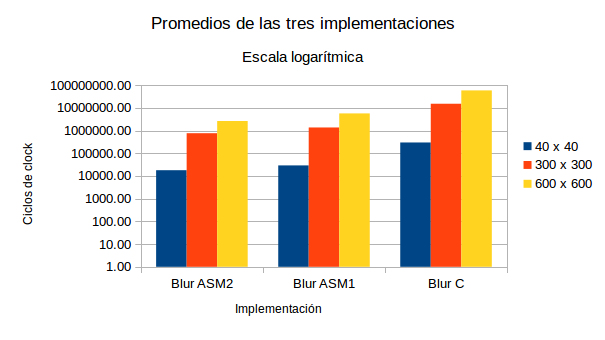
\includegraphics[width=90mm]{blur/graficoBlur.png}
%\caption{A simple caption \label{overflow}}
\end{figure}

Para evaluar si había diferencias en imágenes de un color constante, realizamos los mismos experimentos en este set de caso de pruebas, compuesto con imágenes puramente verdes, azules, rojas, blancas y negras. A continuación, las tablas con resultados de estos experimentos, junto con el gráfico resultante.\\

\begin{tabular}{| l | l | l | l | l |}
\hline
Implementación & Color & 1600 píxeles & 90000 píxeles & 360000 píxeles\\
\hline
Blur ASM1 & Uniforme Blanca & 25158.00 & 1415168.00 & 5707722.00\\ 
\hline
Blur ASM1 & Uniforme Negra & 25008.00 & 1417360.00 & 5821901.00\\ 
\hline
Blur ASM1 & Uniforme Roja & 23542.00 & 1429305.00 & 5522346.00\\ 
\hline
Blur ASM1 & Uniforme Verde & 24259.00 & 1424455.00 & 5663435.00\\
\hline
Blur ASM1 & Uniforme Azul & 23421.00 & 1384261.00 & 5752064.00\\
\hline
Promedio & &  24277.60 & 1414109.80 & 5693493.60\\
\hline
Desvio estándard  &&  803.71 & 17610.73 & 112156.61\\
\hline
Porcentaje de desviación  &&  3.31\% & 1.25\% & 1.97\%\\
\hline
\end{tabular}


\begin{tabular}{| l | l | l | l | l |}
\hline
Implementación & Color & 1600 píxeles & 90000 píxeles & 360000 píxeles\\
\hline
Blur ASM2 & Uniforme Blanca & 13297.00 & 769413.00 & 3180362.00\\ 
\hline
Blur ASM2 & Uniforme Negra & 15364.00 & 777099.00 & 3055456.00\\ 
\hline
Blur ASM2 & Uniforme Roja & 14031.00 & 776847.00 & 3132449.00\\ 
\hline
Blur ASM2 & Uniforme Verde & 16060.00 & 743686.00 & 3191171.00\\
\hline
Blur ASM2 & Uniforme Azul & 14278.00 & 778483.00 & 3159916.00\\
\hline
Promedio & &   14606.00 & 769105.60 & 3143870.80\\
\hline
Desvio estándard  &&  1100.04 & 14645.90 & 54254.03\\
\hline
Porcentaje de desviación  &&   7.53\% & 1.90\% & 1.73\%\\
\hline
\end{tabular}

\begin{tabular}{| l | l | l | l | l |}
\hline
Implementación & Color & 1600 píxeles & 90000 píxeles & 360000 píxeles\\
\hline
Blur C & Uniforme Blanca & 306566.00 & 14236027.00 & 56984192.00\\ 
\hline
Blur C & Uniforme Negra & 303997.00 & 14469139.00 & 56284032.00\\ 
\hline
Blur C & Uniforme Roja & 300376.00 & 14622681.00 & 55996348.00\\ 
\hline
Blur C & Uniforme Verde & 295486.00 & 14840694.00 & 56661072.00\\
\hline
Blur C & Uniforme Azul & 300286.00 & 14917069.00 & 55887204.00\\
\hline
Promedio & &   301342.20 & 14617122.00 & 56362569.60\\
\hline
Desvio estándard  &&  4203.58 & 277090.20 & 458742.02\\
\hline
Porcentaje de desviación  &&   1.39\% & 1.90\% & 0.81\%\\
\hline
\end{tabular}

A partir de esta información, logramos la siguiente tabla que recopila los promedios y nos permite realizar un gráfico comparativo de implementaciones según tamaño.\\



\begin{tabular}{| l | l | l | l|}
\hline
Implementación  & 1600 píxeles & 90000 píxeles & 360000 píxeles\\
\hline
Blur ASM1  & 24277.6 & 1414109.8 & 5693493.6\\
\hline
Blur ASM2  &  14606 & 769105.6 & 3143870.8\\
\hline
Blur C & 301342.2 & 14617122 & 56362569.6\\
\hline
\end{tabular}

\begin{figure}[ht]
\centering
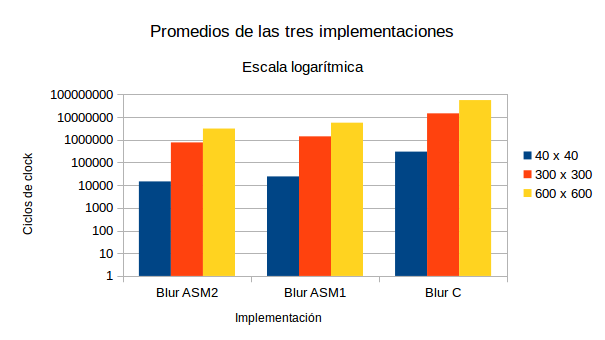
\includegraphics[width=90mm]{blur/graficoBlur_cte.png}
%\caption{A simple caption \label{overflow}}
\end{figure}

\subsubsection{Algunas conclusiones}
Dentro de cada implementación, vemos que el tiempo de ejecución aumenta a medida que aumenta el tamaño de las imágenes de prueba, lo cual era en cierto sentido lo que nos indicaba nuestro intuición que iba a suceder.\\
Así mismo, la implementación más performante resultó ser ASM2.\\
Este resultado no pareciera depender de la cantidad de instrucciones, dado que ambas implementaciones de Assembler poseen una cantidad muy similar de las mismas. 
%todo: me parece que tiene que ver con los accesos a memoria, chequear.
También pudimos corroborar, que para este filtro, el tipo de imagen elegido no afectaba en la performance de la implementación, ya que los porcentajes de desvío son muy pequeños, lo que indica que los promedios de las mediciones de los distintos tipos no se alejan significativamente de la media.\\


